\subsection{Phần hiện thực AI}
\subsubsection{\mbox{Mô hình và công nghệ sử dụng}}
\begin{itemize}
    \item \textbf{\mbox{Mô hình nhúng văn bản:}} Hệ thống sử dụng mô hình 
    \mbox{\texttt{sentence-transformers/paraphrase-multilingual-MiniLM-L12-v2}} 
    để biến đổi dữ liệu văn bản thành các vector nhúng có khả năng biểu diễn ngữ nghĩa, 
    hỗ trợ tốt cả tiếng Việt.
    
    \item \textbf{\mbox{Mô hình nhúng hình ảnh:}} Sử dụng mô hình \mbox{\texttt{clip-ViT-B-32}} 
    (CLIP - Contrastive Language-Image Pre-Training) để chuyển đổi hình ảnh thành 
    các vector nhúng có kích thước chuẩn, cho phép so sánh tương đồng giữa các hình ảnh.
    
    \item \textbf{Công nghệ tìm kiếm vector:} Hệ thống tích hợp FAISS 
    (Facebook AI Similarity Search) để thực hiện tìm kiếm tương tự hiệu quả 
    trên không gian vector, hỗ trợ tìm kiếm nhanh cho cả dữ liệu văn bản và hình ảnh.
    
    \item \textbf{Hệ thống hỏi đáp sản phẩm:} Kết hợp mô hình ngôn ngữ Gemini (Google) 
    với kỹ thuật RAG (Retrieval-Augmented Generation) để trả lời câu hỏi 
    dựa trên thông tin sản phẩm được lưu trữ.
\end{itemize}

\subsubsection{\mbox{Khả năng tìm kiếm bằng hình ảnh}}
\begin{figure}[H]
    \begin{center}
    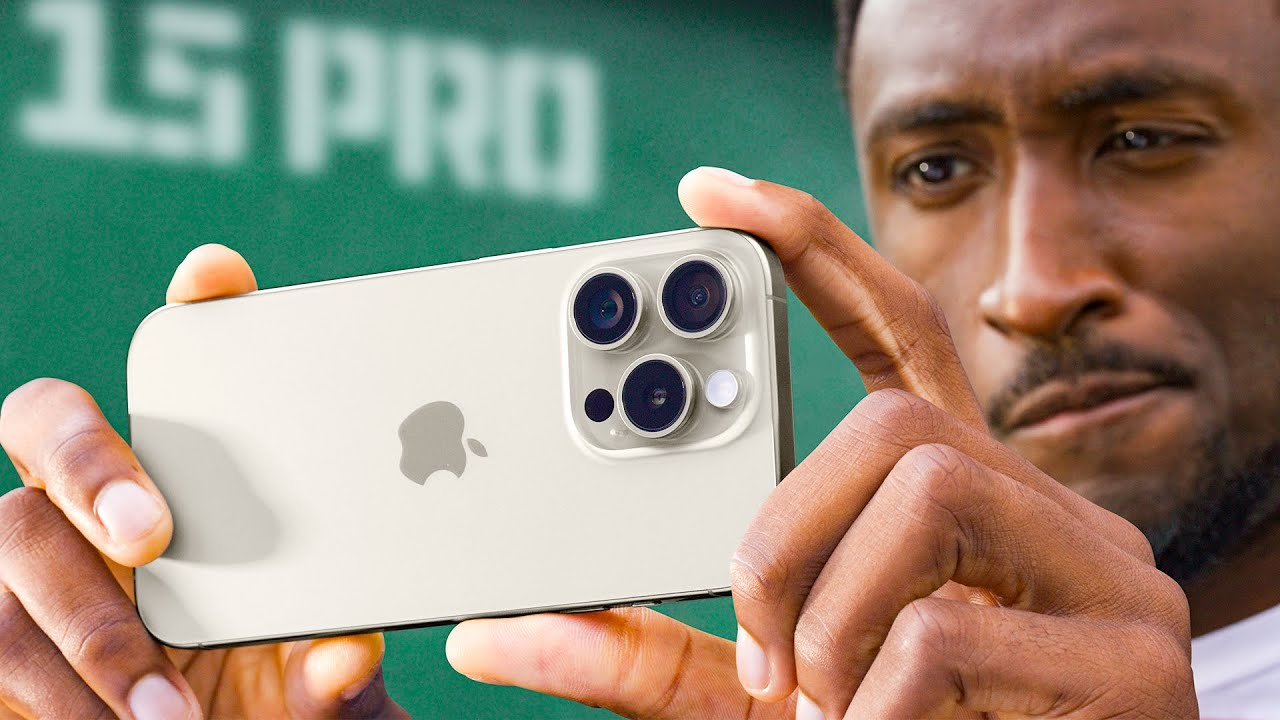
\includegraphics[width=14cm]{component/5. Hiện thực hệ thống/Image/Image/maxresdefault.jpg}
    \end{center}
    \caption{Ảnh test đầu vào}
\end{figure}
\begin{figure}[H]
    \begin{center}
    \includegraphics[width=10cm]{component/5. Hiện thực hệ thống/Image/Admin/AI3.PNG}
    \end{center}
    \caption{Kết quả tìm kiếm tương tự}
\end{figure}

\begin{itemize}
    \item \textbf{Nguyên lý hoạt động:} Hệ thống chuyển đổi hình ảnh đầu vào thành vector nhúng sử dụng mô hình CLIP, sau đó tìm kiếm các sản phẩm có hình ảnh tương tự nhất trong không gian vector sử dụng FAISS.
    
    \item \textbf{Độ tương tự:} Kết quả tìm kiếm kèm theo điểm số tương đồng (similarity score) giữa hình ảnh đầu vào và hình ảnh sản phẩm được tìm thấy, giúp xác định mức độ liên quan.
    
    \item \textbf{Khả năng mở rộng:} Hệ thống dễ dàng cập nhật chỉ mục khi có thêm sản phẩm mới thông qua API \texttt{/refresh-image-index}, đảm bảo luôn cập nhật với dữ liệu sản phẩm mới nhất.
\end{itemize}

\subsubsection{\mbox{Hệ thống hỏi đáp sản phẩm}}
\begin{itemize}
    \item \textbf{\mbox{Kỹ thuật RAG:}} Hệ thống kết hợp giữa khả năng truy xuất thông tin sản phẩm 
    (Retrieval) và khả năng sinh văn bản (Generation) để trả lời câu hỏi người dùng một cách 
    chính xác và có tham chiếu.
    
    \item \textbf{Quy trình xử lý:}
        \begin{enumerate}
            \item Nhận câu hỏi từ người dùng và chuyển đổi thành vector nhúng
            \item Tìm kiếm \texttt{top-k} sản phẩm liên quan nhất trong cơ sở dữ liệu
            \item Trích xuất thông tin chi tiết của các sản phẩm này
            \item Sử dụng mô hình ngôn ngữ Gemini để tổng hợp câu trả lời dựa trên thông tin sản phẩm
        \end{enumerate}
        
    \item \textbf{Khả năng đa ngôn ngữ:} Hỗ trợ cả tiếng Việt và tiếng Anh nhờ vào mô hình nhúng đa ngôn ngữ, đáp ứng nhu cầu đa dạng của người dùng.
\end{itemize}

\subsubsection{\mbox{Tích hợp với cơ sở dữ liệu}}
\begin{itemize}
    \item \textbf{Đồng bộ hóa với MongoDB:} Hệ thống cung cấp API \texttt{/ingest-mongo} để tự động đồng bộ và chỉ mục hóa toàn bộ sản phẩm từ cơ sở dữ liệu MongoDB.
    
    \item \textbf{Xử lý dữ liệu:} Tự động chuyển đổi và chuẩn hóa dữ liệu sản phẩm để tạo vector nhúng chất lượng cao, đảm bảo khả năng tìm kiếm hiệu quả.
    
    \item \textbf{Lưu trữ chỉ mục:} Các chỉ mục FAISS được lưu trữ trên đĩa để tái sử dụng, giảm thiểu thời gian khởi động và tài nguyên hệ thống.
\end{itemize}

\subsubsection{\mbox{Kết luận về tính khả thi}}
\begin{itemize}
    \item \textbf{Hiệu suất:} Hệ thống AI cung cấp khả năng tìm kiếm hình ảnh và hỏi đáp sản phẩm với độ trễ thấp, đáp ứng nhu cầu sử dụng trong ứng dụng thương mại điện tử thời gian thực.
    
    \item \textbf{Khả năng mở rộng:} Kiến trúc dựa trên vector nhúng và chỉ mục FAISS cho phép mở rộng dễ dàng khi số lượng sản phẩm tăng lên, với khả năng xử lý hàng triệu sản phẩm.
    
    \item \textbf{Triển khai thực tế:} Được triển khai như một API RESTful, hệ thống dễ dàng tích hợp vào quy trình tìm kiếm và đề xuất sản phẩm trên nền tảng web hoặc ứng dụng di động, góp phần nâng cao trải nghiệm người dùng.
    
    \item \textbf{Cải tiến tương lai:} Có thể cải thiện thêm bằng cách bổ sung thêm dữ liệu huấn luyện, cập nhật mô hình nhúng mới, và tối ưu hóa các tham số tìm kiếm để tăng độ chính xác và hiệu suất.
\end{itemize}

\subsection{\mbox{Kiểm thử chức năng hệ thống}}

\subsubsection{\mbox{Tính năng xác thực đăng nhập}}
\begin{table}[H]
\centering
\begin{adjustbox}{width=1\textwidth}
\begin{tabular}{|p{0.08\textwidth}|p{0.20\textwidth}|p{0.30\textwidth}|p{0.25\textwidth}|p{0.15\textwidth}|}
\hline
\textbf{ID} & \textbf{Test Case} & \textbf{Dữ liệu test} & \textbf{Kết quả mong đợi} & \textbf{Trạng Thái} \\ \hline
1.1 & Sai tên tài khoản & \begin{tabular}[c]{@{}l@{}}Tài khoản: test \\ Mật khẩu: test\end{tabular} & Không thể đăng nhập vào hệ thống & Thành Công \\ \hline
1.2 & Sai mật khẩu & \begin{tabular}[c]{@{}l@{}}Username: test123 \\ Mật khẩu: test123\end{tabular} & Không thể đăng nhập vào hệ thống & Thành Công \\ \hline
1.3 & Đăng nhập thành công & \begin{tabular}[c]{@{}l@{}}Username: phamkhanhhuy \\ Mật khẩu: Huypham123!\end{tabular} & Đăng nhập vào hệ thống thành công & Thành Công \\ \hline
\end{tabular}
\end{adjustbox}
\caption{Test cases cho tính năng xác thực.}
\label{tab:auth-test-cases}
\end{table}

\subsubsection{\mbox{Tính năng đăng ký}}
\begin{table}[H]
\centering
\begin{adjustbox}{width=1\textwidth}
\begin{tabular}{|p{0.08\textwidth}|p{0.20\textwidth}|p{0.30\textwidth}|p{0.25\textwidth}|p{0.15\textwidth}|}
\hline
\textbf{ID} & \textbf{Test Case} & \textbf{Dữ liệu test} & \textbf{Kết quả mong đợi} & \textbf{Trạng Thái} \\ \hline
2.1 & \begin{tabular}[c]{@{}l@{}}Tạo tài khoản\\thành công\end{tabular} & 
\begin{tabular}[c]{@{}l@{}}Email: test123@gmail.com\\Tên tài khoản: test123\\Mật khẩu: test12\\Xác thực lại mật khẩu: test12\end{tabular} & 
Đăng ký tài khoản thành công & Thành Công \\ \hline
2.2 & \begin{tabular}[c]{@{}l@{}}Trùng tên\\tài khoản đã có\end{tabular} & 
\begin{tabular}[c]{@{}l@{}}Email: test123@gmail.com\\Tên tài khoản: test123\\Mật khẩu: test\\Xác thực lại mật khẩu: test\end{tabular} & 
Đăng ký tài khoản không thành công & Thành Công \\ \hline
\end{tabular}
\end{adjustbox}
\caption{Test cases cho chức năng đăng ký tài khoản.}
\label{tab:register-test-cases}
\end{table}
